\usetikzlibrary{positioning,arrows.meta,calc}
\tikzset
{
  myTrapezium/.pic =
  {
    \draw [fill=blue!40] (0,0) -- (0,\b) -- (\a,\c) -- (\a,-\c) -- (0,-\b) -- cycle ;
    \coordinate (-center) at (\a/2,0);
    \coordinate (-out) at (\a,0);
  },
  myArrows/.style=
  {
    line width=2mm, 
    black,
    -{Triangle[length=1.5mm,width=5mm]},
    shorten >=2.5pt, 
    shorten <=2pt, 
  }
}
    \def\a{4}  % width of trapezium
    \def\b{1.} % small height of trapezium
    \def\c{2.2}  % tall height of trapezium

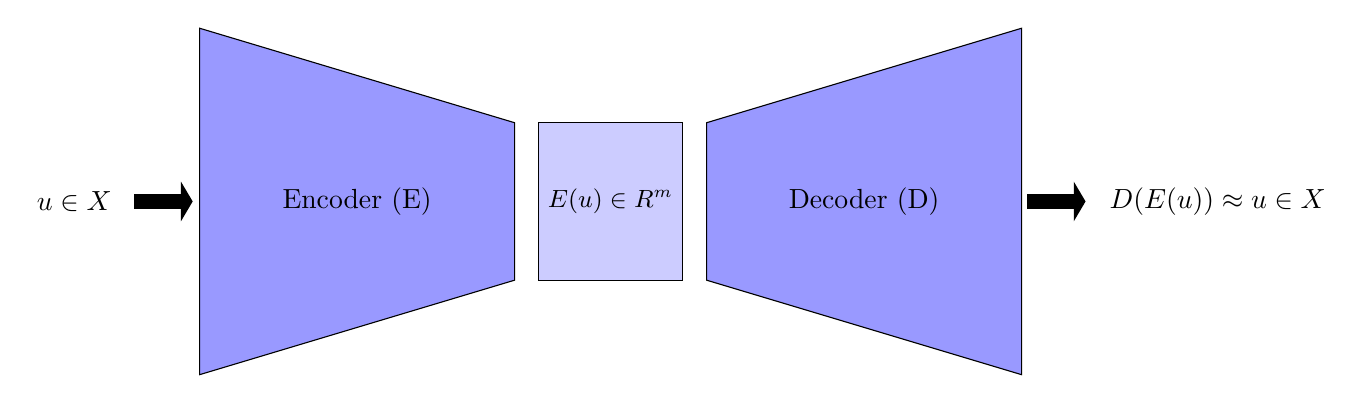
\begin{tikzpicture}
[
  node distance=3mm, % space between drawn parts
  every node/.style={align=center},
]


  \node (middleThing) 
  [
    draw,
    fill=blue!20,
    %minimum width=1cm,
    minimum height=2*\b cm,
    font=\small,
    ]
  {$E(u)\in \mathbb{R}^m$};
  \pic (right)[right=of middleThing.east] {myTrapezium} ;
  \pic (left)[left=of middleThing.west, rotate=180] {myTrapezium} ;
  \node at (right-center) {Decoder (D)} ;
  \node at (left-center) {Encoder (E)};

  \def\d{.9}
  \coordinate (u) at (\d,0);
  \draw [myArrows] (right-out) -- ++(u) node [anchor=west] {$D(E(u))\approx u \in X$} ;
  \draw [myArrows] ($(left-out)-(u)$) node [anchor=east] {$u \in X$} -- ++(u) ;

\end{tikzpicture}
